\section{Results}\label{sec:results}

The experiments test whether adding the frozen \scl{} between an unchanged detector and an
unchanged tracker keeps or improves tracking, on MOT17 and KITTI, on two external trackers, and,
without retuning, on UAVDT. Three outcomes are expected from the design. A tracker that already fits
its detector should keep its accuracy. A tracker that does not fit, because it has no continuation
step or because the detector or its score scale changed, should gain. Both should hold on trackers
and data that were not seen during design.

All experiments use the hosts and detectors of Sect.~\ref{sec:hosts}, each with the authors' code
and published configuration, and the contract of each host is given in Table~\ref{tab:contracts}.
For each host, two systems are compared. The baseline is the host alone (the host-only baseline),
called Host in the tables:
the published tracker without \scl{}, run by us with its published configuration and the same
detections. The second system adds the frozen \scl{} of Sect.~\ref{sec:method} and changes nothing
else. Both runs use the same environment. Where the authors report their own numbers, these are
listed next to our reproduction of the host. Uncertainty is estimated with the paired bootstrap of
Sect.~\ref{sec:metrics}. Figure~\ref{fig:forest} shows the HOTA difference between each host with
\scl{} and the host alone for every tested cell, and the next subsections give the results of each
part of the evaluation.

\begin{figure}[tp]
\centering
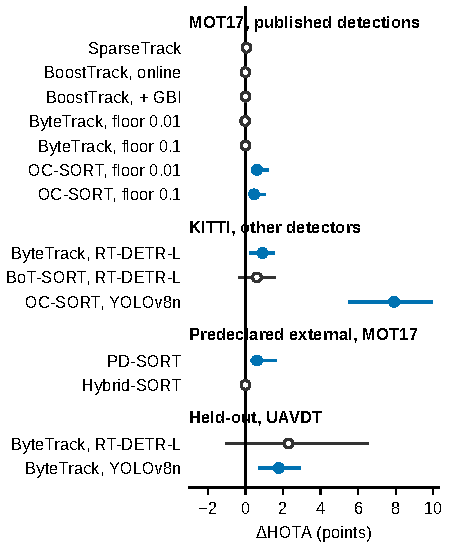
\includegraphics{Fig5.pdf}
\caption{Difference in HOTA, host with \scl{} minus host alone, in points, for
every tested cell. The circle is the difference and the horizontal line its 95\%
paired-bootstrap interval. Filled circles: interval above zero; open circles:
interval contains zero, or identical output}
\label{fig:forest}
\end{figure}

\subsection{MOT17 evaluation across trackers}\label{sec:tracker}
The MOT17 evaluation tests whether \scl{} leaves well-matched trackers at their own accuracy and
helps a tracker that lacks a continuation step, with the published YOLOX-X detections.
Table~\ref{tab:mot17} compares the development trackers with their hosts on MOT17 val-half. The
two-stage trackers with well-matched detections stayed at the accuracy of their hosts. BoostTrack,
online and with GBI, and ByteTrack at floor 0.1 gave exactly the same output as without the layer,
and ByteTrack at floor 0.01 and SparseTrack stayed within 0.06 HOTA points of their hosts
($-0.014$ and $+0.055$). This is the self-limiting behavior of the clean mode
(Sect.~\ref{sec:regimes}), which the earlier design did not have (Table~\ref{tab:prior}).

The single-stage OC-SORT improved at both emission floors. Its HOTA rose by 0.61 points
($[+0.36,+1.24]$) at floor 0.01 and by 0.46 points ($[+0.27,+1.09]$) at floor 0.1, and its MOTA by
1.27 and 1.26 points. Its identity switches also fell, by 8 at floor 0.01 ($[-15,-2]$) and by 14 at
floor 0.1. HOTA was higher on 7 of 7 sequences in both settings (Fig.~\ref{fig:perseq}). The gain
comes from the continuation rescue. OC-SORT drops every detection below its single threshold, and
the layer passes it the foreground candidates that continue a track that would otherwise stay
unmatched.

\begin{table}[tp]
\caption{Baseline comparison of the development trackers on MOT17 val-half
(published YOLOX-X detections). Paper: number reported by the tracker's
authors. Host: the tracker alone, without \scl{} (our run of the published tracker). $\Delta$: host with
\scl{} minus host, with 95\% paired-bootstrap interval (10,000
resamples, seed 42); bold intervals exclude zero. The floor is the lowest
detector score emitted. IDS: identity switches, a count (lower is better);
--: not reported by the authors.}
\label{tab:mot17}
\centering\footnotesize
\setlength{\tabcolsep}{4pt}
\begin{tabular}{@{}lrrl@{}}
\toprule
Metric & Paper & Host & $\Delta$ [95\% CI]\\
\midrule
\multicolumn{4}{@{}l}{\textit{SparseTrack} \cite{liu2025sparsetrack}}\\
\quad HOTA & 69.2 & 68.88 & $+0.06$ [$-0.01$, $+0.25$]\\
\quad MOTA & 76.8 & 77.85 & $+0.08$ [$-0.03$, $+0.30$]\\
\quad IDF1 & 81.4 & 81.97 & $+0.16$ [$-0.02$, $+0.70$]\\
\quad IDS & -- & 124 & $+7$ [$0$, $+19$]\\
\multicolumn{4}{@{}l}{\textit{BoostTrack, online} \cite{stanojevic2024boosttrack}}\\
\quad HOTA & 68.37 & 68.49 & 0 (identical)\\
\quad MOTA & 75.56 & 75.50 & 0 (identical)\\
\quad IDF1 & 81.35 & 81.41 & 0 (identical)\\
\quad IDS & 118 & 113 & 0 (identical)\\
\multicolumn{4}{@{}l}{\textit{BoostTrack, + GBI} \cite{stanojevic2024boosttrack}}\\
\quad HOTA & 71.33 & 71.72 & 0 (identical)\\
\quad MOTA & 80.55 & 81.03 & 0 (identical)\\
\quad IDF1 & 83.84 & 84.16 & 0 (identical)\\
\quad IDS & 106 & 97 & 0 (identical)\\
\multicolumn{4}{@{}l}{\textit{ByteTrack, floor 0.01} \cite{zhang2022bytetrack}}\\
\quad HOTA & -- & 67.70 & $-0.014$ [$-0.058$, $+0.009$]\\
\quad MOTA & 76.6 & 77.60 & $+0.06$ [$-0.15$, $+0.34$]\\
\quad IDF1 & 79.3 & 79.47 & $-0.031$ [$-0.135$, $+0.035$]\\
\quad IDS & -- & 214 & $+4$ [$-2$, $+13$]\\
\multicolumn{4}{@{}l}{\textit{ByteTrack, floor 0.1} \cite{zhang2022bytetrack}}\\
\quad HOTA & -- & 67.70 & 0 (identical)\\
\quad MOTA & 76.6 & 77.60 & 0 (identical)\\
\quad IDF1 & 79.3 & 79.47 & 0 (identical)\\
\quad IDS & -- & 214 & 0 (identical)\\
\multicolumn{4}{@{}l}{\textit{OC-SORT, floor 0.01} \cite{cao2023ocsort}}\\
\quad HOTA & 66.5 & 66.43 & {\boldmath $+0.61$ [$+0.36$, $+1.24$]}\\
\quad MOTA & 74.9 & 74.67 & {\boldmath $+1.27$ [$+0.17$, $+3.01$]}\\
\quad IDF1 & 77.7 & 78.05 & $+0.66$ [$-0.25$, $+1.60$]\\
\quad IDS & -- & 211 & {\boldmath $-8$ [$-15$, $-2$]}\\
\multicolumn{4}{@{}l}{\textit{OC-SORT, floor 0.1} \cite{cao2023ocsort}}\\
\quad HOTA & 66.5 & 66.44 & {\boldmath $+0.46$ [$+0.27$, $+1.09$]}\\
\quad MOTA & 74.9 & 74.67 & {\boldmath $+1.26$ [$+0.37$, $+3.34$]}\\
\quad IDF1 & 77.7 & 78.05 & {\boldmath $+0.287$ [$+0.003$, $+0.838$]}\\
\quad IDS & -- & 213 & $-14$ [$-38$, $+6$]\\
\bottomrule
\end{tabular}
\end{table}


\begin{figure*}[tp]
\centering
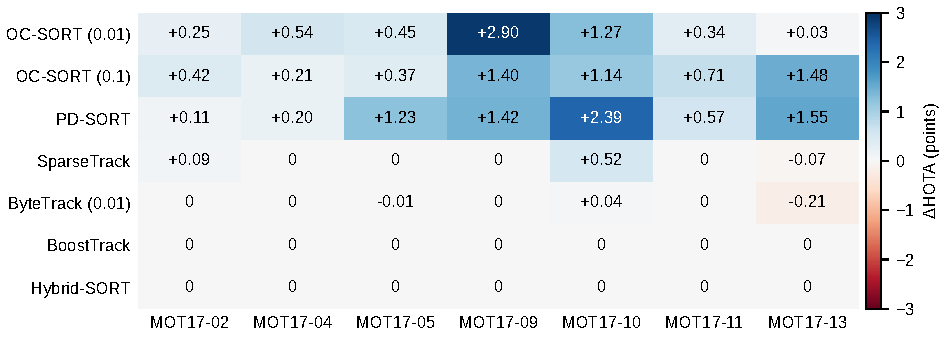
\includegraphics{Fig6.pdf}
\caption{HOTA difference, host with \scl{} minus host alone, in points, for each
MOT17 val-half sequence (columns) and each development or predeclared tracker
(rows). Each cell prints its value; the shade grows with the size of the
difference, and 0 means identical output}
\label{fig:perseq}
\end{figure*}

\subsection{KITTI evaluation with other detectors}\label{sec:detector}
The KITTI evaluation tests what happens when the detector is replaced while each tracker keeps the
thresholds that were set for another detector. Table~\ref{tab:kitti} reports the results with the
two other detectors. With the noisy RT-DETR-L detector, the two-stage trackers gained in MOTA and
IDF1. ByteTrack gained 5.98 MOTA points ($[+1.16,+9.94]$), 3.87 IDF1 points, and 0.91 HOTA points
($[+0.22,+1.55]$). BoT-SORT gained 7.86 MOTA points ($[+2.21,+13.44]$) and 3.10 IDF1 points. Both
also had fewer identity switches: 297 fewer for ByteTrack and 226 fewer for BoT-SORT. With YOLOv8n,
the single-stage OC-SORT gained 7.91 HOTA points ($[+5.47,+9.98]$), 9.40 MOTA points, and 9.60 IDF1
points, the metric of how well identities are kept. It now followed many more objects: its missed
objects (FN) fell by 5,310, from 21,886 to 16,576, and its identity switch count rose with them by
79. Figure~\ref{fig:example} shows one frame of this cell: OC-SORT alone tracked 6 of the 10
labelled objects, and with \scl{} it tracked 9, including parked cars further down the street.

\begin{table}[tp]
\caption{Baseline comparison under a detector change on KITTI tracking
training (official HOTA, car and pedestrian averaged). Host: the tracker
alone, without \scl{}, with the same detections. $\Delta$: host with \scl{}
minus host, with 95\% paired-bootstrap interval; bold intervals exclude zero.
IDS: identity switches, a count (lower is better). BoT-SORT: KITTI sequence 0020
is left out of both runs, because the BoT-SORT code stopped with a numerical
error in its Kalman update on it; the other 20 sequences are used.}
\label{tab:kitti}
\centering\footnotesize
\setlength{\tabcolsep}{4pt}
\begin{tabular}{@{}lrl@{}}
\toprule
Metric & Host & $\Delta$ [95\% CI]\\
\midrule
\multicolumn{3}{@{}l}{\textit{ByteTrack} \cite{zhang2022bytetrack}\textit{, RT-DETR-L}}\\
\quad HOTA & 50.73 & {\boldmath $+0.91$ [$+0.22$, $+1.55$]}\\
\quad MOTA & 47.27 & {\boldmath $+5.98$ [$+1.16$, $+9.94$]}\\
\quad IDF1 & 64.98 & {\boldmath $+3.87$ [$+1.67$, $+5.06$]}\\
\quad IDS & 686 & {\boldmath $-297$ [$-530$, $-122$]}\\
\multicolumn{3}{@{}l}{\textit{BoT-SORT} \cite{aharon2022botsort}\textit{, RT-DETR-L} (20 sequences)}\\
\quad HOTA & 53.91 & $+0.61$ [$-0.39$, $+1.61$]\\
\quad MOTA & 48.25 & {\boldmath $+7.86$ [$+2.21$, $+13.44$]}\\
\quad IDF1 & 67.74 & {\boldmath $+3.10$ [$+1.00$, $+4.57$]}\\
\quad IDS & 476 & {\boldmath $-226$ [$-369$, $-120$]}\\
\multicolumn{3}{@{}l}{\textit{OC-SORT} \cite{cao2023ocsort}\textit{, YOLOv8n}}\\
\quad HOTA & 36.27 & {\boldmath $+7.91$ [$+5.47$, $+9.98$]}\\
\quad MOTA & 33.99 & {\boldmath $+9.40$ [$+1.10$, $+12.30$]}\\
\quad IDF1 & 50.46 & {\boldmath $+9.60$ [$+5.61$, $+12.16$]}\\
\quad IDS & 91 & {\boldmath $+79$ [$+43$, $+125$]}\\
\bottomrule
\end{tabular}
\end{table}


\begin{figure*}[tp]
\centering
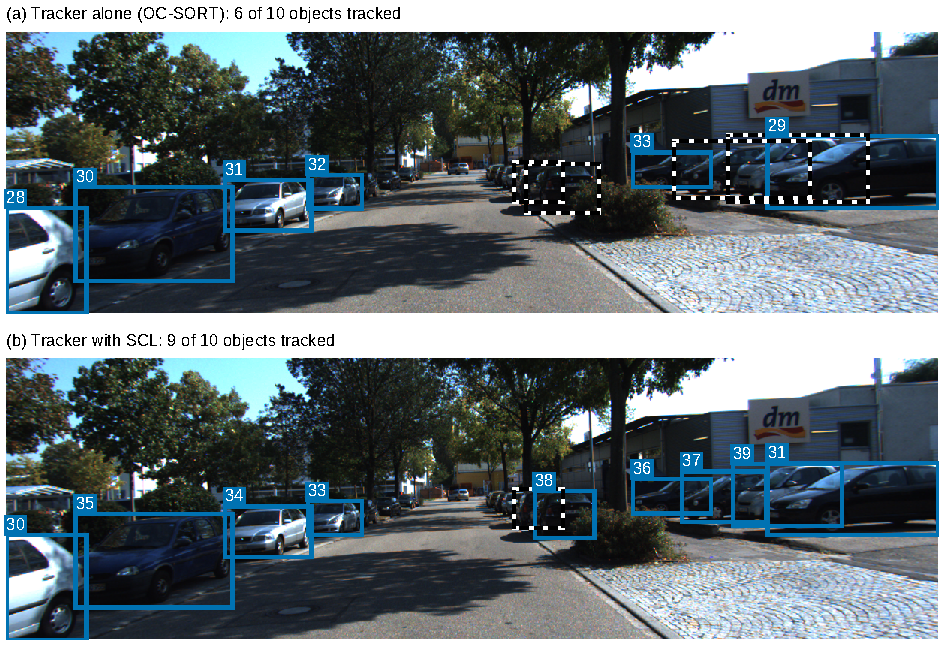
\includegraphics{Fig7.pdf}
\caption{Example frame from KITTI tracking training \cite{geiger2012kitti} (sequence 0001, frame
102), OC-SORT with YOLOv8n detections: (a) the tracker alone, (b) with \scl{}. Solid boxes with
numbers: the tracks output for this frame and their IDs; dashed boxes: labelled cars and
pedestrians that no output box covers. The sequence is the one with the median HOTA gain of the
21 sequences, and the frame is the first one in it with the largest gain in tracked objects}
\label{fig:example}
\end{figure*}

\subsection{Evaluation under shifted detector scores}\label{sec:shift}
The shifted scores test the case for which \scl{} was built: the detector keeps its boxes, but its
score scale changes. Table~\ref{tab:shift} and Fig.~\ref{fig:shift} show the trackers under the four
score transforms of Sect.~\ref{sec:data}. Halving the scores reduced ByteTrack (official setting)
and OC-SORT to 0 HOTA, because no detection reached their thresholds. With the layer they reached
66.17 and 66.72. Cubing reduced them to 60.92 and 58.34, and the layer restored them to 65.81 and
66.60. BoostTrack rose from 61.33 to 64.84 under cubing. With temperature $T=2$, the layer raised
ByteTrack and OC-SORT by 1.11 and 1.24 points. The library setting of ByteTrack, whose low
thresholds already accept the changed scores, stayed within 0.14 points in all four transforms.
Over the 14 conditions, the layer raised HOTA significantly in 7 and lowered it significantly in
none.

\begin{table}[tp]
\caption{Baseline comparison under shifted detector scores on MOT17 val-half. The detector
scores are transformed before the tracker, whose published thresholds stay fixed; $T$ is a logit
temperature, $\sigma(z/T)$. Host: the tracker alone, without \scl{}. $\Delta$: with \scl{} minus host,
with 95\% paired-bootstrap interval (10,000 resamples, seed 42); bold intervals exclude zero.
Emission floor 0.01 (BoostTrack 0.1).}
\label{tab:shift}
\centering\footnotesize
\setlength{\tabcolsep}{4pt}
\begin{tabular}{@{}lrrl@{}}
\toprule
 & \multicolumn{3}{c}{HOTA (\%)}\\
\cmidrule(l){2-4}
Transform & Host & + \scl{} & $\Delta$ [95\% CI]\\
\midrule
\multicolumn{4}{@{}l}{\textit{ByteTrack, official setting} \cite{zhang2022bytetrack}}\\
\quad $s^3$ & 60.92 & 65.81 & {\boldmath $+4.89$ [$+2.60$, $+13.69$]}\\
\quad $0.5\,s$ & 0.00 & 66.17 & {\boldmath $+66.17$ [$+49.32$, $+75.40$]}\\
\quad $T=2$ & 65.84 & 66.95 & {\boldmath $+1.11$ [$+0.35$, $+3.87$]}\\
\quad $T=0.5$ & 67.30 & 67.29 & $-0.009$ [$-0.051$, $+0.005$]\\
\multicolumn{4}{@{}l}{\textit{ByteTrack, library setting} \cite{zhang2022bytetrack}}\\
\quad $s^3$ & 66.31 & 66.31 & $-0.006$ [$-0.384$, $+0.383$]\\
\quad $0.5\,s$ & 66.61 & 66.48 & $-0.14$ [$-0.66$, $+0.14$]\\
\quad $T=2$ & 63.97 & 63.97 & 0 (identical)\\
\quad $T=0.5$ & 66.53 & 66.52 & $-0.006$ [$-0.029$, $+0.001$]\\
\multicolumn{4}{@{}l}{\textit{OC-SORT} \cite{cao2023ocsort}}\\
\quad $s^3$ & 58.34 & 66.60 & {\boldmath $+8.26$ [$+5.86$, $+16.81$]}\\
\quad $0.5\,s$ & 0.00 & 66.72 & {\boldmath $+66.72$ [$+50.32$, $+75.56$]}\\
\quad $T=2$ & 65.99 & 67.22 & {\boldmath $+1.24$ [$+0.52$, $+3.42$]}\\
\quad $T=0.5$ & 66.61 & 67.06 & $+0.45$ [$-0.01$, $+0.97$]\\
\multicolumn{4}{@{}l}{\textit{BoostTrack, online} \cite{stanojevic2024boosttrack}}\\
\quad $s^3$ & 61.33 & 64.84 & {\boldmath $+3.51$ [$+0.85$, $+13.28$]}\\
\quad $T=2$ & 67.59 & 67.59 & 0 (identical)\\
\bottomrule
\end{tabular}
\end{table}


\begin{figure*}[tp]
\centering
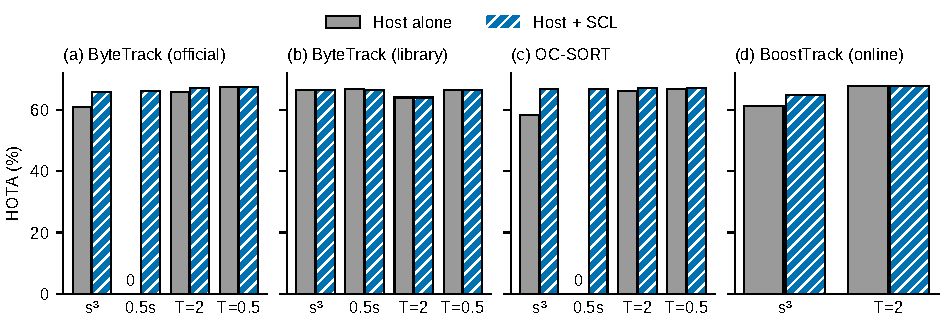
\includegraphics{Fig8.pdf}
\caption{Shifted detector scores on MOT17 val-half: HOTA of each published
tracker with its published thresholds, alone and with \scl{}, after
four monotone transforms of the detector scores ($s^3$, $0.5\,s$, and
temperatures $T=2$ and $T=0.5$). (a) ByteTrack, official setting;
(b) ByteTrack, library setting; (c) OC-SORT; (d) BoostTrack, online. Plain bars: the
tracker alone; hatched bars: with \scl{}}
\label{fig:shift}
\end{figure*}

\subsection{Comparison with adaptive-threshold methods}\label{sec:baselines}
A simpler way to follow the detector scores is to set the tracker's thresholds from them directly.
Two such baselines were built on the same input and with the same window of the last 10 frames.
They set the tracker's matching and birth thresholds in every frame to the first or the second Otsu
split of the recent logits, $t_1$ or $t_2$, and pass the scores unchanged, without the mode
decision, the new scores, or the rescue. Table~\ref{tab:baselines} compares them with \scl{} on
KITTI, for OC-SORT with YOLOv8n and for both trackers under halved scores. \scl{} reached the
highest HOTA in all three cells, 2.2 to 8.6 points above the two baselines, and its paired-bootstrap
intervals against the $t_2$ baseline lie above zero in every cell. Adaptive thresholds alone
therefore do not explain the gains; the other parts of the layer add to them. With OC-SORT,
\scl{} also had fewer identity switches than both baselines, with YOLOv8n (170 against 1,545 and
250) and under halved scores (308 against 1,975 and 492).

\emph{Comparison with a published method.} ACT \cite{act2026adaptive} sets the high and low
thresholds of a two-stage tracker in every frame from the first quartile and the number of the
current scores, using fixed score levels. It was run with its published parameters on the same
detections as \scl{}, in three settings (Table~\ref{tab:act}): KITTI with halved scores, for
ByteTrack and, with its high threshold as the single threshold, for OC-SORT; its own setting, MOT17
val-half with ByteTrack's official setting and the YOLOX-X detections; and the held-out UAVDT test
split with ByteTrack. \scl{} reached higher HOTA than ACT in every row of Table~\ref{tab:act}. The
difference was significant under halved scores ($+2.01$ and $+10.06$ points) and with YOLOv8n on
UAVDT ($+1.82$ points, with $+4.00$ points of IDF1). In the setting for which ACT was designed,
\scl{} was also higher ($+0.22$ and $+0.23$ points). With RT-DETR-L on UAVDT, \scl{} reached a MOTA of 27.99 against
5.34 for ACT (difference $+22.65$, [$+9.03$, $+47.21$]): the host produced many false positives,
and the fixed levels of ACT removed few of them (178,219 false positives, against 78,975 with
\scl{}). \scl{} also had fewer identity switches than ACT on MOT17 (18 and 22 fewer) and UAVDT (185 and
418 fewer), significantly with RT-DETR-L on UAVDT. Under halved scores on KITTI, it missed far fewer objects than ACT:
7,750 against 12,326 with ByteTrack, and 13,547 against 21,887 with OC-SORT. The levels of ACT are fixed scores, so they do not move when the
scores shift, while the splits of \scl{} are computed on the scores themselves.

\emph{Contribution of each part.} Removing one part of the frozen \scl{} at a time shows where the
gains come from, on the KITTI cells. Without the continuation rescue, the HOTA of OC-SORT fell by
3.34 points with YOLOv8n and by 1.16 points under halved scores. Using the clean mode in every
frame, that is, without the mode decision, lowered HOTA by 0.90 points for ByteTrack with RT-DETR-L
and by 2.40 and 2.44 points for the two trackers under halved scores. Without the new scores of the
noisy mode, HOTA fell by 1.67 and 0.61 points under halved scores.

\begin{table}[tp]
\caption{HOTA (\%) of \scl{} and of two simple adaptive-threshold baselines on KITTI tracking
training (official HOTA, car and pedestrian averaged). Host: the tracker alone, without any layer.
$t_1$, $t_2$: the adaptive baselines, in which the tracker's matching and birth thresholds are set in every frame to the
first or second Otsu split of the logits of the last 10 frames, and the scores are passed unchanged.
Halved: halved detector scores. $\Delta$: \scl{} minus the $t_2$ baseline, with 95\% paired-bootstrap interval below the
value; bold intervals exclude zero.}
\label{tab:baselines}
\centering\footnotesize
\setlength{\tabcolsep}{3pt}
\begin{tabular}{@{}lrrrrc@{}}
\toprule
Cell & Host & $t_1$ & $t_2$ & \scl{} & $\Delta$\\
\midrule
\twol{OC-SORT,}{YOLOv8n} & 36.27 & 39.97 & 41.09 & 44.17 & \cib{+3.09}{+2.00}{+4.03}\\
\addlinespace[3pt]
\begin{tabular}[c]{@{}l@{}}ByteTrack,\\RT-DETR-L,\\halved\end{tabular} & 49.50 & 49.58 & 49.50 & 51.78 & \cib{+2.29}{+0.28}{+4.96}\\
\addlinespace[3pt]
\begin{tabular}[c]{@{}l@{}}OC-SORT,\\YOLOv8n,\\halved\end{tabular} & 0.00 & 37.68 & 43.56 & 46.30 & \cib{+2.74}{+1.32}{+3.34}\\
\bottomrule
\end{tabular}
\end{table}

\begin{table*}[tp]
\caption{HOTA of ACT \cite{act2026adaptive} and of \scl{} on the same detections, and the
differences \scl{} minus ACT in HOTA and IDF1, with 95\% paired-bootstrap interval below each
value; bold intervals exclude zero. ACT: published parameters, no
tuning. KITTI: official HOTA, car and pedestrian averaged; MOT17: val-half, ACT's own setting;
UAVDT: test split, one vehicle class, ignored regions removed (Sect.~\ref{sec:metrics}).}
\label{tab:act}
\centering\footnotesize
\setlength{\tabcolsep}{5pt}
\begin{tabular}{@{}lllrrcc@{}}
\toprule
Data & Detector & Tracker & ACT & \scl{} & $\Delta$HOTA & $\Delta$IDF1\\
\midrule
KITTI, halved scores & RT-DETR-L & ByteTrack & 49.77 & 51.78 & \cib{+2.01}{+0.01}{+4.76} & \ci{+1.70}{-1.13}{+6.80}\\
KITTI, halved scores & YOLOv8n & OC-SORT & 36.24 & 46.30 & \cib{+10.06}{+6.88}{+12.01} & \cib{+12.03}{+6.85}{+14.69}\\
\addlinespace[4pt]
MOT17, floor 0.01 & YOLOX-X & ByteTrack (official) & 67.46 & 67.68 & \ci{+0.22}{-0.43}{+0.88} & \ci{+0.57}{-0.68}{+2.12}\\
MOT17, floor 0.1 & YOLOX-X & ByteTrack (official) & 67.46 & 67.70 & \ci{+0.23}{-0.40}{+0.90} & \ci{+0.60}{-0.55}{+2.10}\\
\addlinespace[4pt]
UAVDT test & YOLOv8n & ByteTrack & 29.01 & 30.83 & \cib{+1.82}{+0.65}{+3.00} & \cib{+4.00}{+1.85}{+6.22}\\
UAVDT test & RT-DETR-L & ByteTrack & 40.14 & 42.37 & \ci{+2.23}{-0.97}{+6.32} & \ci{+5.35}{-0.03}{+12.47}\\
\bottomrule
\end{tabular}
\end{table*}


\subsection{Frozen evaluation on external trackers}\label{sec:external}
The external evaluation tests whether the frozen \scl{} helps trackers that were not seen during
design. Table~\ref{tab:external} gives the two predeclared external systems. PD-SORT
\cite{wang2025pdsort} was reproduced exactly as in the authors' released output. With \scl{}, its
HOTA rose by 0.61 points ($[+0.27,+1.65]$), its MOTA by 1.13 points ($[+0.27,+3.03]$), and its IDF1
by 0.82 points ($[+0.43,+1.94]$), with higher HOTA on 7 of 7 sequences (Fig.~\ref{fig:perseq}). FN
fell by 1,291, and the identity switches stayed almost the same (131 against 129).
PD-SORT is a single-stage tracker, and its gain comes from the same step as for OC-SORT; unlike
OC-SORT, it was not seen during design. Hybrid-SORT \cite{yang2024hybridsort}, a two-stage tracker,
gave identical output, as predicted before the run.

\begin{table}[tp]
\caption{Baseline comparison on the predeclared external systems (MOT17
val-half, authors' released detections), each evaluated once with the frozen
\scl{}. Paper: number reported by the authors (for PD-SORT, their released
output). Host: the tracker alone, without \scl{} (our run of the published tracker). Reproduction class
against the authors' number (EXACT: $|\Delta\mathrm{HOTA}|\le0.2$; CLOSE:
$\le1.0$ with a documented, untuned cause). $\Delta$: host with \scl{} minus
host, with 95\% paired-bootstrap interval; bold intervals exclude zero. IDS:
identity switches, a count (lower is better); --: not reported.}
\label{tab:external}
\centering\footnotesize
\setlength{\tabcolsep}{4pt}
\begin{tabular}{@{}lrrl@{}}
\toprule
Metric & Paper & Host & $\Delta$ [95\% CI]\\
\midrule
\multicolumn{4}{@{}l}{\textit{PD-SORT} \cite{wang2025pdsort}\textit{, EXACT}}\\
\quad HOTA & 68.01 & 68.01 & {\boldmath $+0.61$ [$+0.27$, $+1.65$]}\\
\quad MOTA & 75.19 & 75.19 & {\boldmath $+1.13$ [$+0.27$, $+3.03$]}\\
\quad IDF1 & 81.03 & 81.03 & {\boldmath $+0.82$ [$+0.43$, $+1.94$]}\\
\quad IDS & -- & 129 & $+2$ [$-9$, $+13$]\\
\multicolumn{4}{@{}l}{\textit{Hybrid-SORT} \cite{yang2024hybridsort}\textit{, CLOSE}}\\
\quad HOTA & 67.1 & 66.70 & 0 (identical)\\
\quad MOTA & 75.8 & 75.52 & 0 (identical)\\
\quad IDF1 & 78.0 & 77.56 & 0 (identical)\\
\quad IDS & -- & 259 & 0 (identical)\\
\bottomrule
\end{tabular}
\end{table}


\subsection{Frozen UAVDT transfer}\label{sec:visdrone}
The UAVDT transfer tests whether the frozen \scl{} still helps on aerial data that was not used
during design, with none of its values changed. It uses the 20 test sequences of
Sect.~\ref{sec:data}, and each cell was run once with the frozen configuration.
Table~\ref{tab:visdrone} gives the results. \scl{} raised the HOTA of the YOLOv8n stream by 1.77
points ($[+0.70,+2.94]$) and its IDF1 by 3.97 points ($[+1.88,+6.17]$), and identity switches fell
by 45\% (from 719 to 393). With RT-DETR-L, the host produced many false positives (MOTA 3.29); with
\scl{}, its MOTA rose by 24.70 points ($[+10.06,+51.08]$) and its IDF1 by 5.74 points
($[+0.13,+13.11]$): false positives fell by 58\% and identity switches by 56\% (from 1,041 to 455).
HOTA did not fall with either detector.

\begin{table}[tp]
\caption{Baseline comparison on the held-out UAVDT test split (20 aerial
sequences, not used during design), evaluated once with the frozen \scl{}. Host: ByteTrack alone, without \scl{}, with its published setting. $\Delta$: host
with \scl{} minus host, with 95\% paired-bootstrap interval; bold intervals
exclude zero. IDS: identity switches, a count (lower is better).}
\label{tab:visdrone}
\centering\footnotesize
\setlength{\tabcolsep}{4pt}
\begin{tabular}{@{}lrl@{}}
\toprule
Metric & Host & $\Delta$ [95\% CI]\\
\midrule
\multicolumn{3}{@{}l}{\textit{ByteTrack, RT-DETR-L} \cite{zhang2022bytetrack,zhao2024rtdetr}}\\
\quad HOTA & 40.07 & $+2.30$ [$-1.05$, $+6.55$]\\
\quad MOTA & 3.29 & {\boldmath $+24.70$ [$+10.06$, $+51.08$]}\\
\quad IDF1 & 48.59 & {\boldmath $+5.74$ [$+0.13$, $+13.11$]}\\
\quad IDS & 1041 & {\boldmath $-586$ [$-951$, $-248$]}\\
\multicolumn{3}{@{}l}{\textit{ByteTrack, YOLOv8n} \cite{zhang2022bytetrack,jocher2023yolov8}}\\
\quad HOTA & 29.05 & {\boldmath $+1.77$ [$+0.70$, $+2.94$]}\\
\quad MOTA & 16.27 & $+1.02$ [$-1.06$, $+2.86$]\\
\quad IDF1 & 34.52 & {\boldmath $+3.97$ [$+1.88$, $+6.17$]}\\
\quad IDS & 719 & {\boldmath $-326$ [$-691$, $-73$]}\\
\bottomrule
\end{tabular}
\end{table}

